\documentclass[12pt, a4paper]{article}

\usepackage{lastpage}
\usepackage{mathtools}
\usepackage{xltxtra}
\usepackage{libertine}
\usepackage{amsmath}
\usepackage{amsthm}
\usepackage{amsfonts}
\usepackage{amssymb}
\usepackage{enumitem}
\usepackage{xcolor}
\usepackage[left=1.5cm, right=1.5cm, top=2cm, bottom=2cm, bindingoffset=0cm, headheight=15pt]{geometry}
\usepackage{fancyhdr}
\usepackage[russian]{babel}
% \usepackage[utf8]{inputenc}
\usepackage{catchfilebetweentags}
\usepackage{accents}
\usepackage{calc}
\usepackage{etoolbox}
\usepackage{mathrsfs}
\usepackage{wrapfig}

\providetoggle{useproofs}
\settoggle{useproofs}{false}

\pagestyle{fancy}
\lfoot{M3137y2019}
\rhead{\thepage\ из \pageref{LastPage}}

\newcommand{\R}{\mathbb{R}}
\newcommand{\Q}{\mathbb{Q}}
\newcommand{\C}{\mathbb{C}}
\newcommand{\Z}{\mathbb{Z}}
\newcommand{\B}{\mathbb{B}}
\newcommand{\N}{\mathbb{N}}

\newcommand{\const}{\text{const}}

\newcommand{\teormin}{\textcolor{red}{!}\ }

\DeclareMathOperator*{\xor}{\oplus}
\DeclareMathOperator*{\equ}{\sim}
\DeclareMathOperator{\Ln}{\text{Ln}}
\DeclareMathOperator{\sign}{\text{sign}}
\DeclareMathOperator{\Sym}{\text{Sym}}
\DeclareMathOperator{\Asym}{\text{Asym}}
% \DeclareMathOperator{\sh}{\text{sh}}
% \DeclareMathOperator{\tg}{\text{tg}}
% \DeclareMathOperator{\arctg}{\text{arctg}}
% \DeclareMathOperator{\ch}{\text{ch}}

\DeclarePairedDelimiter{\ceil}{\lceil}{\rceil}
\DeclarePairedDelimiter{\abs}{\left\lvert}{\right\rvert}

\setmainfont{Linux Libertine}

\theoremstyle{plain}
\newtheorem{axiom}{Аксиома}
\newtheorem{lemma}{Лемма}

\theoremstyle{remark}
\newtheorem*{remark}{Примечание}
\newtheorem*{exercise}{Упражнение}
\newtheorem*{consequence}{Следствие}
\newtheorem*{example}{Пример}
\newtheorem*{observation}{Наблюдение}

\theoremstyle{definition}
\newtheorem{theorem}{Теорема}
\newtheorem*{definition}{Определение}
\newtheorem*{obozn}{Обозначение}

\setlength{\parindent}{0pt}

\newcommand{\dbltilde}[1]{\accentset{\approx}{#1}}
\newcommand{\intt}{\int\!}

% magical thing that fixes paragraphs
\makeatletter
\patchcmd{\CatchFBT@Fin@l}{\endlinechar\m@ne}{}
  {}{\typeout{Unsuccessful patch!}}
\makeatother

\newcommand{\get}[2]{
    \ExecuteMetaData[#1]{#2}
}

\newcommand{\getproof}[2]{
    \iftoggle{useproofs}{\ExecuteMetaData[#1]{#2proof}}{}
}

\newcommand{\getwithproof}[2]{
    \get{#1}{#2}
    \getproof{#1}{#2}
}

\newcommand{\import}[3]{
    \subsection{#1}
    \getwithproof{#2}{#3}
}

\newcommand{\given}[1]{
    Дано выше. (\ref{#1}, стр. \pageref{#1})
}

\renewcommand{\ker}{\text{Ker }}
\newcommand{\im}{\text{Im }}
\newcommand{\grad}{\text{grad}}

\lhead{Конспект по матанализу}
\cfoot{}
\rfoot{Лекция 11}

\renewcommand{\thesubsection}{\arabic{subsection}.}

\begin{document}

\begin{theorem}
    Интегральный признак Коши.

    $f:[1, +\infty)\to\R$ монотонно убывает, $f\geq 0, f$ непр.

    Тогда $\sum_{k=1}^\infty f(k)$ и $\int_1^{+\infty} f(x)dx$ сходится/расходится одновременно.
\end{theorem}
\begin{proof}
    $$\sum_{k=1}^n f(k) = \int_1^{n+1} f(x)dx + \Delta_n$$
    \begin{figure}[h]
        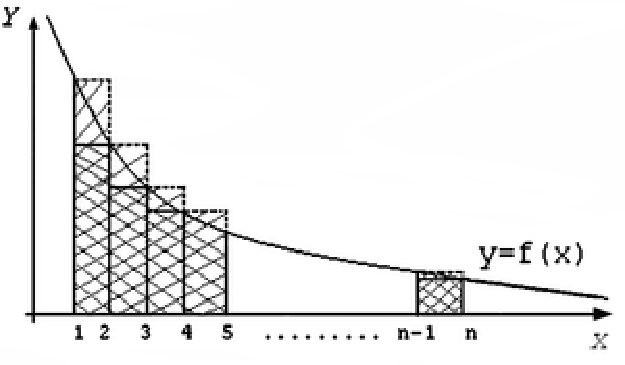
\includegraphics[scale=0.6]{images/cauchy.pdf}
        \centering
    \end{figure}

    $\Delta_n$ --- площадь криволинейных треугольников, получаемых отсечением кривой $y=f(x)$.

    $$0 \le \Delta_n \le f(1) - f(n) \le f(1)$$
    $\Delta_n\uparrow \Rightarrow \exists$ кон. $\lim \Delta_n$

    Более формальный вариант, без картинок:
    $$\sum_{k=1}^n - \int_1^{n+1} = \sum_{k=1}^n\left(f(k) - \int_k^{k+1} f(x)dx \right)$$
    Т.к. $f\downarrow$:
    $$\int_k^{k+1} f(x)dx \ge \int_k^{k+1} f(k+1)dx=f(k+1)$$
    $$\sum_{k=1}^n\left(f(k) - \int_k^{k+1} f(x)dx \right) \le \sum_{k=1}^n f(k) - f(k+1) = f(1) - f(n+1)$$
\end{proof}

\begin{example}
    $\sum \frac{1}{k^\alpha (\ln k)^\beta}$
    
    Способы:
    \begin{enumerate}
        \item ``Удавить логарифм'' % себя удави
        \item Покажем, что $\frac{1}{k^\alpha (\ln k)^\beta}$ монотонна НСНМ:
        $$f' = \frac{-\alpha}{x^{\alpha+1}(\ln x)^\beta} - \frac{\beta}{x^{\alpha+1}(\ln x)^\beta \ln x}\equ\limits_{x\to+\infty} \frac{-\alpha}{x^{\alpha+1}(\ln x)^\beta} \Rightarrow f'<0 \text{ НСНМ}$$

        Перейдем к интегралу:
        $$\int_2^{+\infty} \frac{1}{x^\alpha (\ln x)^\beta} dx$$
        \begin{itemize}
            \item $\alpha > 1$ сходится
            \item $\alpha < 1$ расходится
            \item $\alpha = 1$: \begin{itemize}
                \item $\beta > 1$ сходится
                \item $\beta \le 1$ расходится
            \end{itemize}
        \end{itemize}
        По другим признакам сходимость ряда нельзя выяснить.
    \end{enumerate}
\end{example}

\begin{definition}
    Ряд $A$ \textbf{абсолютно сходится}, если 1 и 2:
    \begin{enumerate}
        \item $\sum a_n$ сх.
        \item $\sum |a_n|$ сх.
    \end{enumerate}
\end{definition}

\begin{example}
    $$\frac{1}{1+x^2}=1-x^2+x^4-\ldots+(-1)^nx^{2n} + \frac{(-1)^{n+1} x^{2n+2}}{1+x^2}$$
    Возьмём интеграл на $[0, 1]$:
    $$\frac{\pi}{4} = 1 - \frac{1}{3} + \frac{1}{5} - \ldots \frac{(-1)^n}{2n+1} + \underbrace{\int_0^1 \frac{(-1)^{n+1}x^{2n+2}}{1+x^2}dx}_{\Delta_n}$$
    Устремим $n\to+\infty$
    $$\frac{\pi}{4}=1-\frac{1}{3}+\frac{1}{5}-\frac{1}{7}+\frac{1}{9}+\ldots$$
    Таким образом, мы посчитали сумму ряда, это ряд Лейбница. По модулю этот ряд не сходится.
\end{example}

\begin{theorem}
    $\sum a_n, a_n\in\R$. Тогда эквивалентны следующие утверждения:
    \begin{enumerate}
        \item $\sum a_n$ абс. сх.
        \item $\sum |a_n|$ сх.
        \item Оба ряда $\sum a_n^+, \sum a_n^-$ сх. 
    \end{enumerate}
\end{theorem}

\section*{Сходимость рядов \textcolor{red}{\ldots}}

\begin{theorem}
    Признак Лейбница.

    $c_n\ge 0, c_1\ge c_2\ge c_3 \ge \ldots, c_n\to 0$

    Тогда $\sum_{n=1}^{+\infty} (-1)^n c_n$ сх.
\end{theorem}
\begin{proof}
    $$S_{2N}=c_1-c_2+\ldots + c_{2N-1}-c_{2N}$$
    $$S_{2N+2}=S_{2N}+(c_{2N+1}-c_{2N+2})\geq S_{2N}$$
    $$S_{2N}\uparrow, S_{2N}\leq c_1$$
\end{proof}

\begin{remark}
    Секретное приложение к признаку Лейбница.

    В условиях признака Лейбница:
    $$\left|\sum_{n=N}^{+\infty} (-1)^{n-1}C_n\right| \le |C_n|$$
\end{remark}

\begin{example}
    $$\sum_{k=1}^{+\infty} \frac{(-1)^k}{\sqrt k + (-1)^k}$$
    $$c_k=\frac{1}{\sqrt k + (-1)^k}$$
    Не монотонно.
\end{example}

Для незнакостабильных рядов признак эквивалентности не работает.

\section*{Функции и отображения в $\R^m$}

\subsection{Структуры в $\R^m$}

\begin{itemize}
    \item Линейное пространство $x=(x_1\ldots x_m), x_i\in\R$. Строка/столбец --- не важно.
    
    $$\langle x,y\rangle=\sum_{i=1}^m x_iy_i$$
    
    $$|x|=\sqrt{\langle x,x\rangle}=\sqrt{\sum x_i^2}$$
    
    $$\rho(x,y):=|x-y|$$

    \item Окрестности, шар
    
    $B(a, r)=\{x\in\R^m : |x-a|<r\}$ --- открытый шар, $r$-окрестность точки $a$

    Открытые множества, замкнутые множества.

    Внутренняя точка, предельная точка множества.

    \item Сходимость, предел
    
    $$x_n\to a, x_n \text{ --- посл. в } \R^m, a\in\R^m$$

    $$\forall U(a) \ \ \exists \ \ N \ \ \forall n > N \ \ x_n\in U(a)$$

    $$x_n\to a, y_n\to b \Rightarrow \langle x_n, y_n\rangle \to \langle a,b\rangle$$
    
    % $f : O\subset \R^m \to \R^n$

    % $a$ --- предельная точка $O$, $L\in \R^n$

    % $\lim\limits_{x\to a} f(x) = L$

    \textcolor{red}{Немного скипнуто}

    В $\R^m$ комп. $\Leftrightarrow$ замкн. и огр.

    Секвенциальная компактность: $\forall (x_n), x_n\in K \Rightarrow \exists n_k, a\in K : x_{n_k}\to a$

    Применение компактности : принцип выбора Больцано-Вейерштрасса, теорема Вейерштрасса.
\end{itemize}

$$\lim_{y\to0, x\to0} \frac{x+y}{x-y}=\lim_{y\to0} \lim_{x\to0} \frac{x+y}{x-y}=\lim_{y\to0} -1$$
$$=\lim_{x\to0} \lim_{y\to0} \frac{x+y}{x-y} = \lim 1 = 1$$
Получили противоречие. Что мы сделали не так?

\begin{theorem}
    О повторных пределах

    $D_1, D_2\in\R$, $a$ --- пр. точка $D_1$, $b$ --- пр. точка $D_2$

    $D=(D_1\setminus\{a\})\times(D_2\setminus \{b\})$

    Пусть:
    \begin{enumerate}
        \item $\exists \lim\limits_{(x,y)\to (a,b)} f(x, y)=A\in\overline\R$
        \item $\forall x \in D_1\setminus\{a\} \ \ \exists$ кон. $\varphi(x) = \lim\limits_{y\to b} f(x, y)$
    \end{enumerate}
    Тогда $\exists \lim\limits_{x\to a} \varphi(x)=A$
\end{theorem}

\begin{proof}
    Пусть $A\in\R$
    $$\forall \varepsilon > 0 \ \ \exists \delta>0 \ \ \forall x \in D_1 \ \ |x-a|<\delta$$
    $$\forall \varepsilon > 0 \ \ \exists \delta>0 \ \ \forall y \in D_2 \ \ |y-b|<\delta$$
    $$|f(x,y) - A| < \varepsilon \xRightarrow{y\to b} |\varphi(x)-A|\le \varepsilon$$
\end{proof}

\begin{example}
    $f(x,y)=(x+y)\sin\frac{1}{x}\sin\frac{1}{y}$

    $D=\R^2 \setminus (\{\text{ось } Ox\}\cup \{\text{ось } Oy\})$

    $$\lim_{(x,y)\to(0,0)}\underbrace{(x+y)}_{\text{б.м.}}\underbrace{\sin\frac{1}{x}\sin\frac{1}{y}}_{\text{огр.}}=0$$
    $$\varphi(x) = \lim_{y\to0}\underbrace{(x+y)}_{\to x}\sin\frac{1}{x}\underbrace{\sin\frac{1}{y}}_{\not\exists\lim}$$
\end{example}

Загадка:
$$f(x, y) = \frac{xy}{x^2+y^2}$$
$$\lim_{x\to0}\lim_{y\to0}\frac{xy}{x^2+y^2}=\lim 0 = 0$$
По теореме если предел $\exists$, то он $=0$. Но существует ли он?

\end{document}